\section{Comparison to Prior Work}
\label{sec:comparison}

\subsection{UQLM and multi-sample methods}
\label{subsec:uqlm}

UQLM~\cite{uqlm2024}'s \texttt{BlackBoxUQ} samples each prompt 5
times and scores semantic disagreement via a DeBERTa NLI model.

\begin{table}[h]
\centering
\small
\begin{tabular}{lrrrr}
\toprule
Method & HIGH det. & LOW FP & API calls & Localization \\
\midrule
UQLM (confidence $<0.5$)  & $5\%$  & $0\%$  & $5$ & File-level only \\
\eps (\textsc{flagged+})   & $85\%$ & $50\%$ & $1$ & Token/line/function \\
\bottomrule
\end{tabular}
\caption{UQLM vs.\ \eps on GPT-4o. UQLM returned confidence $\ge 0.62$
on 29/30 prompts (19/20 HIGH); its sole detection (pandas
\texttt{concat}) is a case where syntax genuinely varied across
samples.}
\label{tab:uqlm}
\end{table}

\textbf{UQLM's 0\% false-positive rate reflects the absence of signal,
not the presence of precision} --- a system that never fires achieves
perfect FPR trivially. Lowering the threshold does not recover
detection: LOW prompts fire before additional HIGH do. The Stripe
scenario makes this concrete: the model assigned $0.52/0.47$ to
\texttt{.Charge}/\texttt{.PaymentIntent} at generation time, yet
across 5 samples picked \texttt{PaymentIntent} every time (a
$0.52$-peaked distribution samples its peak nearly always). UQLM
observes perfect consistency and reports confidence $=1.0$. For
intra-generational uncertainty, measuring at the output level cannot
recover the signal by construction.

\begin{figure}[H]
\centering
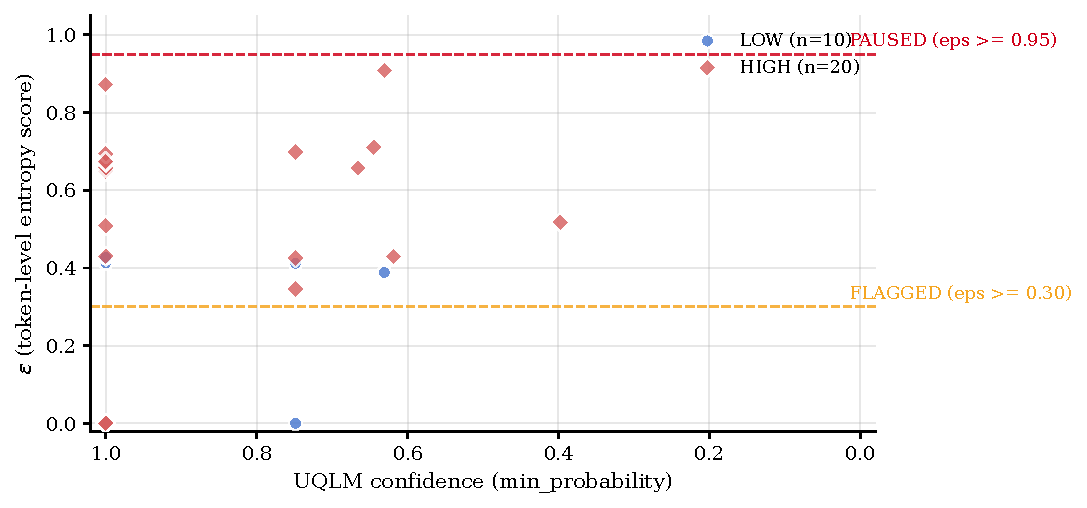
\includegraphics[width=0.85\textwidth]{figures/fig1_scatter.pdf}
\caption{UQLM returned confidence $\ge 0.62$ on $29/30$ prompts
(including $19/20$ HIGH). Its sole detection is pandas \texttt{concat},
where syntax genuinely varied across samples; $\eps$ separates the
two populations by construction.}
\label{fig:scatter}
\end{figure}

\begin{figure}[H]
\centering
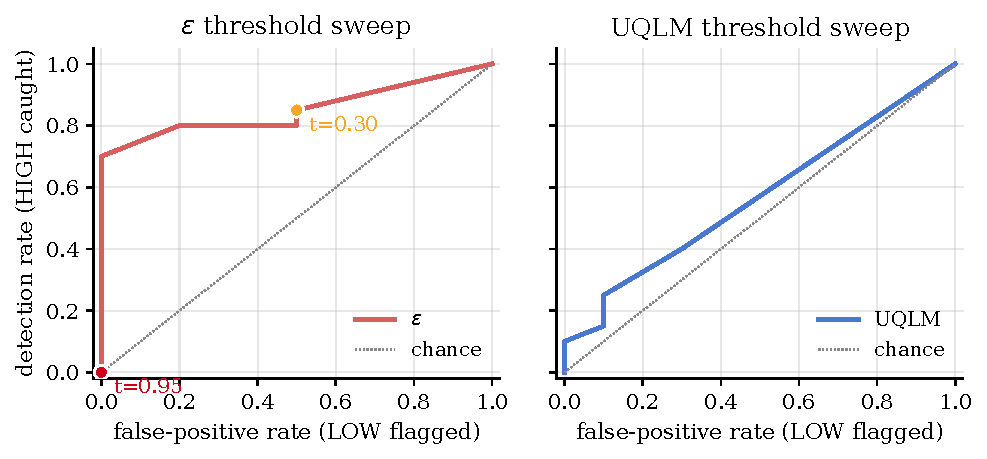
\includegraphics[width=\textwidth]{figures/fig5_roc_sweep.pdf}
\caption{Sweeping the decision threshold for each method on GPT-4o.
$\eps$ has a wide band where HIGH detection dominates LOW FP; UQLM's
useful operating range collapses as threshold rises.}
\label{fig:roc-sweep}
\end{figure}

\subsection{Single-token log-probability baselines}
\label{subsec:logprob}

\texttt{min\_logprob} flags a function if any selected token's
log-probability falls below a threshold --- same raw signal, top-$1$
only.

\begin{table}[h]
\centering
\small
\begin{tabular}{lrr}
\toprule
Method & HIGH det.\ @ $30\%$ LOW FP & HIGH det.\ @ $50\%$ LOW FP \\
\midrule
\texttt{min\_logprob}       & $45$--$55\%$ & $55$--$65\%$ \\
\eps (max, AST-filtered)    & $\mathbf{70\%}$ & $\mathbf{85\%}$ \\
\bottomrule
\end{tabular}
\caption{Matched LOW FP budgets across four models. Gap is at
near-tie tokens (e.g., $0.48/0.42$): \texttt{min\_logprob} sees $0.48$
and does not fire; \eps sees near-uniform top-$k$ entropy and does.}
\label{tab:logprob}
\end{table}

A low top-$1$ probability does not distinguish a cosmetic name from
an API selector from a whitespace artifact. AST filtering plus top-$k$
entropy closes the gap: the signal is in the raw logprobs, inaccessible
without filtering.

\subsection{Static analysis, linters, and model coverage}
\label{subsec:static-cov}

Static analysis catches \emph{known}-bad patterns for libraries with
rules written; \eps fires where the model itself hesitated, including
decisions not yet in any ruleset (a library updated last week, a
half-migrated codebase). Static analysis is the floor under \eps.
Primary experiments use OpenAI plus DeepSeek V3 via Together AI;
Anthropic exposes logprobs via streaming, vLLM via full top-$k$. The
method requires only top-$k$; no model-internal access.
